
\documentclass[a4paper,fleqn,usenatbib]{mnras}

\usepackage{newtxtext,newtxmath}
% Depending on your LaTeX fonts installation, you might get better results with one of these:
%\usepackage{mathptmx}
%\usepackage{txfonts}

\usepackage[T1]{fontenc}
\usepackage{ae,aecompl}
\usepackage{booktabs}


\usepackage{graphicx}	% Including figure files
\usepackage{amsmath}	% Advanced maths commands
\usepackage{amssymb}	% Extra maths symbols
\usepackage{color}

%%%%%%%%%%%%%%%%%%%%%%%%%%%%%%%%%%%%%%%%%%%%%%%%%%

%%%%% AUTHORS - PLACE YOUR OWN COMMANDS HERE %%%%%
\usepackage{float}
\newcommand{\todo}[1]{\textcolor{red}{#1}}
\newcommand{\countertodo}[1]{\textcolor{green}{#1}}

\makeatletter
\newcommand{\rmnum}[1]{\romannumeral #1}
\newcommand{\Rmnum}[1]{\expandafter\@slowromancap\romannumeral #1@}
\makeatother

\title[S-process stars in LAMOST]{Discovery of s-process stars in the LAMOST survey}

\author[B.~J. Norfolk et al.]{B.~J. Norfolk,$^{1}$\thanks{E-mail: bjee7@student.monash.edu (MU)}
A.~R. Casey,$^{1,2}$
M.~T. Miles,$^{1}$
A.~J. Kemp,$^{1}$ 
A.~I. Karakas,$^{1}$ \newauthor
J.~C. Lattanzio,$^{1}$
K.~C. Schlaufman,$^{3}$
and A.~Y.~Q. Ho$^{4}$
\\
$^{1}$School of Physics \& Astronomy, Monash University, Clayton 3800, Victoria, Australia\\
$^{2}$Faculty of Information Technology, Monash University, Clayton 3800, Victoria, Australia\\
$^{3}$Department of Physics and Astronomy, Johns Hopkins University, 3400 N Charles St., Baltimore, MD 21218, USA\\
$^{4}$Cahill Center for Astrophysics, California Institute of Technology, MC 249-17, 1200 E California Blvd, Pasadena, Ca, 91125, USA
}
\date{Accepted XXX. Received YYY; in original form ZZZ}

\pubyear{2018}

\begin{document}
\label{firstpage}
\pagerange{\pageref{firstpage}--\pageref{lastpage}}
\maketitle

\begin{abstract}
Stars with peculiar enhancements of carbon and heavy elements ($Z > 30$) are historically referred to as `Barium stars'. While this chemical abundance pattern can be explained by thermally pulsing asymptotic giant branch (AGB) stars, many so-called Barium stars have not evolved through the red giant phase and therefore cannot be AGB stars. These less-evolved stars are generally thought to have accreted mass from a more-evolved AGB companion. For this reason the frequency and properties of less-evolved Barium stars are uniquely informative on the binary fraction, AGB yields, mass transfer, and stellar evolution. Here we present the discovery of 967 s-process candidates from 454,180 giant stars observed by LAMOST. Our sample includes; 257 `Barium stars' that show enhancement in both barium and strontium, 49 stars showing only significant barium enhancement, and 661 exhibiting only strontium enhancement. This sample constitutes the largest number of s-process enhanced stars ever discovered, and represents the most comprehensive search for Barium stars in the Milky Way. All of our Barium stars are consistent with membership in the Milky Way disk, and we find an \todo{steady/increasing/decreasing} fraction of Barium stars with stellar metallicity, as \todo{expected} from AGB yields and stellar evolution theory. We find up to 51 Barium stars exhibit some evidence of technetium from LAMOST spectra, and most (46/51) have $\log{g}>2$, which suggests they cannot be AGB stars and may indicate a recent ($<1\,\textrm{Myr}$) mass accretion event. Most (178/257) Barium stars in our sample show strong carbon enhancement, consistent with the literature. However, despite previous claims indicating that Barium stars are preferentially enhanced in sodium due to the NeNa nucleosynthesis cycle occurring in massive AGB stars, only 5 ($<2$\,\%) of our Barium stars show any evidence of enhancement in sodium. A comparison with AGB yields suggests that the majority of our sample are consistent with a bottom-heavy IMF.
% and highlights a small percentage of intrinsic Barium stars present in our sample. 
When binary properties become available from end-of-mission Gaia astrometry, this sample of s-process stars will be critical in explaining mass transfer in binary systems and refining AGB yields across a range of masses and metallicities.
\end{abstract}

\begin{keywords}
keyword1 -- keyword2 -- keyword3
\end{keywords}

\section{Introduction} \label{sec:intro}

Barium stars as first recognised by \citet{Bidelman1951}, are chemically unique objects that exhibit envelopes with an overabundance of carbon and heavy elements (Z > 30) in comparison to the Sun. Barium stars exist as either intrinsic or extrinsic objects; intrinsic Barium stars are in the TP-AGB (thermally pulsing-asymptotic giant branch) phase, where the overabundance of both carbon and heavy elements are produced through the s-process and exist on the surface as the result of a thermal pulsing cycle. According to the mass-transfer hypothesis, extrinsic Barium stars are a consequence of stellar wind accretion \citep{boffin1988,jorissen1992} or Roche-lobe overflow \citep{webbink1986}, and are within a binary system containing a previous TP-AGB companion star (intrinsic Barium star) in its final phase as a white dwarf \citep{bohm1980,bohm1984}. In fact, \citet{mcclure1983} determines 85\% of all Barium stars are in binary systems and claims that those that appear singular are actually pole-on, or highly eccentric binaries with significant radial velocity variations only occurring in a small phase range as detailed by \citet{pourbaix2004}. For these reasons, the properties and occurrence rate of Barium stars are informative of the theoretical birth rate of AGB stars, the binary star fraction as a function of metallicity, the mass ratio of binary stars, as well as AGB yields across different masses and metallicities. 

The slow neutron capture process (s-process), occurring in the interior of AGB stars, synthesises roughly half of all elements heavier than iron \citep[e.g.,][]{busso1999,travaglio2001,herwig2005,romano2010,kobayashi2011,prantzos2012,bisterzo2014,karakas12016}. Late in the AGB phase, during the thermally pulsing-AGB (TP-AGB) phase, thermal instabilities occur in the He shell every $10^5$ years or so, depending on the H-exhausted core mass. These energy bursts drive a convective zone that sweeps the entire region lying between the core mass and He-shell; mixing the products of nucleosynthesis within these regions. The energy from the thermal pulses force the star to expand, pushing the H-shell out to cooler regions and allowing the convective envelope to move inwards to regions previously mixed by the thermal pulse driven convective zones. This expansion and resulting inward movement is described as the third dredge up (TDU), and is theorised to occur after each thermal pulse. During the TP-AGB phase, enrichment on the surface in $^{12}$C and heavy elements produced by the s-process is a result of the repeated downwash extensions of TDU \citep[e.g.,][]{busso2001}. The star contracts PDU and reignites the H-shell producing the majority of the surface luminosity for the next interpulse period. The interpulse, thermal pulse, and dredge up cycle may occur numerous times and is dependent on the initial mass, composition, and mass-loss rate of the star.

Barium giants form within a metallicity-dependent initial mass range (approximately $0.8 - 8\,M_{\odot}$), with the minimum mass for core helium and carbon burning decreasing as metallicity decreases. The age of these stars vary considerably, with some as old as $\approx$12\,Gyr in metal-poor globular clusters. In contrast, metal-rich, young observable stars may only reach $\approx$100Myr, this includes stars that are at the core carbon burning limit or very close to it \citep[e.g.,][]{whitelock2013}.

Many Barium stars have been discovered in the disk and halo of the Milky Way \citep{gomez1997,mennessier1997}. 
%These studies show that the stellar populations of Barium stars can be separated into two groups when considering their absolute luminosity, kinematic, and spatial properties. 
The relationship between Barium stars in the halo \citep[e.g.,][]{junqueira2001,drake2008,pereira2009,allen2006} and metal-poor, yellow, symbiotic halo stars has been established by \citet{jorissen2005} and \citet{pereira2009}. Additionally, \citet{pereira2011} concludes that metal-rich Barium stars share similar kinematics to other metal-rich and super metal-rich stars already analysed, suggesting that they do not belong to the bulge population. Furthermore, it is necessary to establish known abundances of s-process elements in a greater sample of Barium stars in order to compare their birth rate to theoretical expectations \citep{han1995}, explore the binary fraction at different metallicities, and compare to AGB star yields at different masses and metallicities.

In this paper we analyse 454,180 giant stars from the second LAMOST data release \citep{luo2015} to identify 967 s-process candidates. In Section \ref{sec:methods} we describe the observations and candidate selection, as well as the analysis of high-resolution follow-up observations obtained for a few candidates. In Section \ref{sec:dis} we discuss the properties of our Barium stars in context of existing literature. We provide concluding remarks in Section \ref{sec:con}.

\section{Methods} \label{sec:methods}
\subsection{LAMOST analysis}
\subsubsection{Data-driven analysis}
The LAMOST (Large sky Area Multi-Object Fibre Spectrographic) survey released low-resolution ($\mathcal{R} \approx 1800$) optical spectra (3700\,\AA\ to 9000\,\AA) for over two million stars in their second data release \citep{luo2015}. Stellar parameters ($T_{\rm eff}$, $\log{g}$, [M/H], [$\alpha$/M]) were derived using a data-driven model constructed using high fidelity APOGEE labels of 9,952 giant stars in common between LAMOST and the APOGEE survey \citep{ho2017}. This data-driven model was used to estimate stellar labels for 454,180 giant stars. We note that this sample is exclusively giant stars, implying that we would not identify dwarf s-process enhanced stars. Cross-validation experience shows that the typical uncertainties are about 70\,K in effective temperature $\rm T_{\rm eff}$, 0.1\,dex in surface gravity $\log{g}$, 0.1\,dex in metallicity [M/H], and 0.04\,dex in the $\alpha$-element abundance relative to overall metallicity [$\alpha$/M]. These uncertainties are approximately comparable to the APOGEE uncertainties \citep{alam2015}.


\subsubsection{Candidate selection} \label{sec:cand}
The Barium stars analysed in this research were obtained by filtering for significant flux residuals, taken as, a disparity between the normalised LAMOST flux and the data driven model derived by \citet{ho2017}. Specifically, we identified Barium stars by searching for \ion{Ba}{II} and \ion{Sr}{II} enhancement at the 4554\,\AA\ and 4077\,\AA\ wavelengths, respectively. A negative residual, as shown in a candidate Barium star in Figure \ref{fig:figure1}, illustrates an enhancement in \ion{Ba}{II} and \ion{Sr}{II} at lines 4554\,\AA\, 4077\,\AA. These \ion{Ba}{II} and \ion{Sr}{II} resonance lines are very strong, allowing us to identify stars enhanced in neutron-capture elements given a well-fit model for the data. Stars identified to just show high levels of barium (and not necessarily strontium) required enhancement at both the 4554\,\AA\ and 4934\,\AA\ \ion{Ba}{II} resonance lines, and for stars just enhanced in strontium we looked for significant residuals at the 4554\,\AA\ and 4215\,\AA\ absorption lines.  

We used five filters that each spectrum, for each set of absorption lines, had to meet in order to be considered a s-process candidate; these included:

\renewcommand\labelenumi{(\roman{enumi})}
\renewcommand\theenumi\labelenumi

\begin{enumerate} 
\item Profile amplitude for both enhancement lines must be $A < -0.05$.
\item Both amplitudes must be measured within 3$\sigma$ ($|A|/\sigma _A$ < 3).
\item The wavelength at each absorption line must be within 2\,\AA\ ($\lambda$ < 2).
\item The reduced $\chi^2$ from \emph{The Cannon} must be $\chi_r^2 < 3$.
\item And finally, the LAMOST spectra must have a signal-to-noise ratio of $S/N > 30\,\textrm{pixel}^{-1}$.
\end{enumerate}
In addition, a visual inspection was undertaken to exclude any results containing, false positives, candidates exhibiting data reduction issues, apparent absorption finer then the spectral resolution, and overly noisy normalised LAMOST spectra. This combined method generated 967 s-process candidates including; 257 `Barium stars' enhanced in both barium and strontium, 49 stars exhibiting exclusively barium enhancement, and 661 exhibiting exclusively strontium enhancement, as listed in Table \ref{table:table1}. 

For the remainder of this paper we restrict our analysis to the 257 classical `Barium stars' stars that show enhancement in both barium and strontium. While the 49 or 661 stars with only barium or strontium enhancements (respectively) may also be bonafide barium stars, there may be other explanations for their chemical abundance pattern \citep[e.g.,][]{maiorca2011}, and so we restrict our inferences to a gold sample of Barium stars. Nevertheless, this sample still constitutes the largest collection of Barium stars ever discovered.\todo{cite the next biggest one or two samples}






\begin{figure*}
	% To include a figure from a file named example.*
	% Allowable file formats are eps or ps if compiling using latex
	% or pdf, png, jpg if compiling using pdflatex
	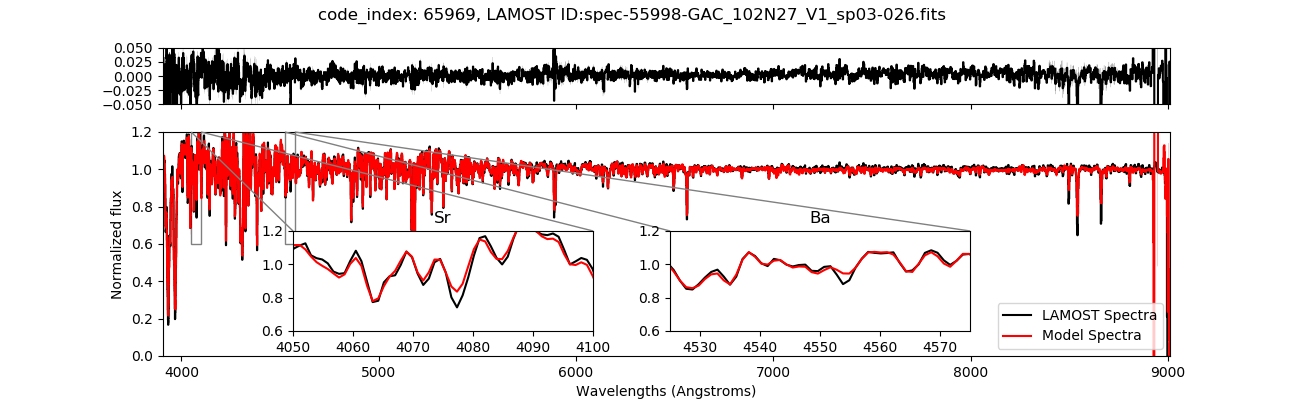
\includegraphics[width=\textwidth]{posterchild.png}
    \caption{Pseudo-continuum-normalised LAMOST spectra for the s-process candidate \todo{CANDIDATENAME}. The data are shown in black and the best-fitting data-driven model is shown in red. We include zoom-in axes to show significant deviations in Sr and Ba at  4077\,\AA\ and 4554\,\AA\, respectively.}
    \label{fig:figure1}
\end{figure*}

\begin{table*}
\centering
\caption{Table is available online in its entirety. Here we show a portion to demonstrate its style and content.}
\label{table:table1}
\begin{tabular}{@{}|l|l|c|c|c|c|c|c|c|c|c|c|c|c|@{}}
\toprule
2MASSID             & R.~A.         & Dec.        & $v_{r}$ & S/N & $\rm T_{\rm eff}$ & $\log{g}$ & [Fe/H] & [$\alpha$/Fe] & $\chi_r^2$ & \ion{Ba}{II}? & \ion{Sr}{II}? & Tc?  \\
& (J2000) & (J2000) & (km\,s$^{-1}$) & (pixel$^{-1}$) & (K)  \\ \midrule
J000134.95+490743.2 & 00:01:34.96 & +49:07:43.2 & $-$42.3    & 72  & 5044 & 3.11  & $-$0.54      & $+$0.11      & 0.79 \\
J000403.80+160257.1 & 00:04:03.80 & +16:02:57.2 & $-$35.4    & 42  & 5200 & 3.40  & $-$0.41      & $+$0.09      & 0.33 \\
J000908.48+421615.4 & 00:09:08.49 & +42:16:15.5 & $-$34.8    & 36  & 4825 & 3.02  & $-$0.46      & $+$0.16      & 0.25 \\
J001754.17+394140.0 & 00:17:54.17 & +39:41:40.0 & $-$42.9    & 39  & 5008 & 3.16  & $-$0.64      & $+$0.12      & 0.23 \\
J001841.57+040533.7 & 00:18:41.57 & +04:05:33.8 & $-$20.7    & 141 & 4840 & 3.68  & $-$0.52      & $+$0.06      & 0.93 \\
J002107.60+361533.0 & 00:21:07.60 & +36:15:33.1 & $-$53.1    & 44  & 4854 & 2.87  & $+$0.01      & $+$0.06      & 0.54 \\
J002537.59+411123.7 & 00:25:37.59 & +41:11:23.8 & $-$12.6    & 36  & 5075 & 3.30  & $-$0.32      & $+$0.10      & 0.33 \\
J003755.55+571706.8 & 00:37:55.55 & +57:17:06.9 & $-$5.7     & 49  & 4046 & 1.14  & $-$0.09      & $-$0.01      & 0.83 \\
J003813.23+423025.9 & 00:38:13.23 & +42:30:25.9 & $-$40.2    & 36  & 4475 & 2.12  & $+$0.14      & $+$0.00      & 0.51 \\
J003959.14+394614.6 & 00:39:59.14 & +39:46:14.6 & $+$5.1     & 35  & 4955 & 3.23  & $-$0.40      & $+$0.11      & 0.28 \\
J004119.68+324627.8 & 00:41:19.68 & +32:46:27.9 & $+$4.5     & 122 & 4861 & 2.59  & $-$0.31      & $+$0.08      & 1.67 \\
J004156.56+390945.6 & 00:41:56.57 & +39:09:45.6 & $-$254.5   & 44  & 4771 & 2.34  & $-$0.74      & $+$0.16      & 0.57 \\
J004743.01+433358.1 & 00:47:43.02 & +43:33:58.2 & $-$62.7    & 65  & 4834 & 2.64  & $-$0.60      & $+$0.17      & 1.06 \\
J005101.98+314045.6 & 00:51:01.98 & +31:40:45.7 & $-$23.7    & 98  & 5202 & 3.32  & $-$0.53      & $+$0.10      & 0.67 \\
J005254.69+203554.7 & 00:52:54.69 & +20:35:54.7 & $+$35.7     & 113 & 5026 & 3.17  & $-$0.82     & $+$0.20      & 1.01 \\
J010836.26+444435.9 & 01:08:36.26 & +44:44:35.9 & $+$12.6     & 49  & 5189 & 3.19  & $-$0.56     & $+$0.10      & 0.98 \\
J011919.20+195227.0 & 01:19:19.21 & +19:52:27.0 & $-$35.4    & 31  & 4897 & 2.77  & $-$0.54      & $+$0.11      & 0.29 \\
J011930.90-015027.3 & 01:19:30.91 & -01:50:27.4 & $-$143.3   & 44  & 5040 & 3.22  & $-$0.91      & $+$0.20      & 0.48 \\
J020316.40+462211.1 & 02:03:16.41 & +46:22:11.1 & $+$11.1     & 37  & 4897 & 2.89  & $-$0.39     & $+$0.11      & 0.51 \\ \bottomrule
\end{tabular}
\end{table*}


\subsubsection{Enhancements due to sodium, technetium, and carbon}
We performed an identical analysis to the process described in Section \ref{sec:cand} in order to identify sodium, technetium, or carbon enhancement in our sample of 257 Barium stars. We used the sodium doublet lines at 5889\,\AA\ and 5895\,\AA\ to select Barium stars enhanced in sodium, and required significant absorption in both features. Only 5/257 Barium stars met this criteria.

For technetium enhancement we searched for significant residual deviations at the 4049\,\AA, 4238\,\AA, 4262\,\AA, 4297\,\AA, and 5924\,\AA. These absorption lines are extremely weak, and would require a substantial amount of technetium before it would be visible in a high S/N LAMOST spectrum. We found 51 Barium stars exhibited some level of significant enhancement (based on the filters above) at a single technetium line, yet none showed enhancement at more than one technetium line. We note that the single enhancement near technetium for these 51 stars may be the consequence of data reduction/calibration artefacts, but we include details of which stars matched on technetium in Table \ref{table:table1} nonetheless.
Finally, for carbon enhancement we searched for significant deviations at the CH and G band near 4300\,\AA. We found 178/257 stars to show significant carbon enhancement (e.g., $[\textrm{C/Fe}] \gtrsim 0.5$).

\subsubsection{Abundance analysis from LAMOST spectra}
We estimated [Ba/Fe] and [Sr/Fe] abundance ratios for all s-process candidates by synthesising spectra that would account for the observed flux residuals. We assumed that absorption due to metals is captured by \emph{The Cannon} model, and deviations in flux at the 4554\,\AA\ \ion{Ba}{II} line and the 4077\,\AA\ \ion{Sr}{II} transition are solely due to enhancements in Ba and Sr, respectively\citep{marcs,sme,vald,ispec}. We adopted the stellar parameters ($T_{\rm eff}$, $\log{g}$, [Fe/H]) from \citep{ho2017}, and assume a microturbulence of $v_{mic} = 2\,{\rm km\,s}^{-1}$. Uncertainties in [Ba/Fe] and [Sr/Fe] from LAMOST are taken as the fitting error due to noise, added in quadrature with an adopted $0.2\,{\rm dex}$ systematic error floor.


\subsection{Follow-up observations with Magellan/MIKE}

\subsubsection{Observations}
On the night of \todo{X} January 2018 we performed follow-up observations of \todo{X} Barium star candidates using the MIKE spectrograph on the Magellan Clay telescope at Las Campanas Observatory, Chile. Candidates for follow-up observations were chosen based on observability constraints and ranked by their apparent visual magnitude. We observed \todo{X} stars in good seeing using the 0.7 arcsecond slit and 2x2 spatial on-chip binning, which provides a spectral resolution of ($\mathcal{R} \approx \todo{22,000}$). Exposure times were set to achieve a S/N ratio of 30 per pixel at 4500\,\AA. We acquired calibration (biases, milky, quartz, and Th-Ar arc lamp) frames in the afternoon.

We reduced the data using the \texttt{CarPy} Python package \citep{kelson2000,kelson2003}. We used spline functions to continuum-normalise individual echelle orders, and resampled the normalised spectra onto a uniform-sized wavelength map. We used a rest-frame normalised template of a FGK-type star to place the observed spectra in the rest frame.


\subsubsection{Abundance analysis}
We adopted the stellar parameters ($T_{\rm eff}$, $\log_{10}g$, [Fe/H]) provided from the data-driven analysis of \citep{ho2017}. Following the procedure outlined in \citep{casey2014}, we measured the strength of atomic absorption lines by fitting Gaussian profiles to the continuum-normalised spectra. Most elemental abundances were derived directly from these line measurements, except for elements that show significant hyperfine splitting \todo{(e.g., )} or blending \todo{(e.g., X)}. In these situations, we adopted a spectral synthesis approach. \todo{citations for line lists}


\todo{Some sentences for our fearless leader to add regarding abundance analysis and verification of stellar parameters from LAMOST}

%\subsubsection{Abundance Uncertainties}

\subsection{Dynamics}
We integrated galactic orbits for 21 Barium stars using recent astrometry from Gaia/TGAS \citep{gaia2016a,gaia2016b}. Using the \texttt{gala} Python package, we integrated each star backwards for $0.5\,\textrm{Gyr}$ in a Milky Way-like potential that consists of four components: a \citet{hernquist1990} bulge and nucleus, a \citet{miyamoto1975} disk, and the \citet{nfw1997} halo. In this potential, the disk and bulge parameters were adjusted to be consistent with previous work \citep{bovy2015}, and to vary the scale mass and radius, of the nucleus and halo, respectively. We computed orbital periods, energy, apocenters, pericenters, eccentricities, and angular momentum in the $z$-direction. All 21 stars showed prograde orbits that were consistent with membership in the Milky Way disk.

\section{Discussion}  \label{sec:dis}


\subsection{Extrinsic and intrinsic Barium stars}
Barium stars exist as either intrinsic or extrinsic objects. Intrinsic Barium stars must be massive enough to reach the TP-AGB phase, and extrinsic Barium stars must be in a binary with a previously polluting TP-AGB star companion. Figure \ref{fig:figure2} shows that the majority of our Barium stars have $\log{g} > 2$, highlighting that most stars in our sample are not massive enough to have already reached the TP-AGB phase and therefore, must be extrinsic Barium stars. The classification for Barium stars with $\log{g} < 2$ is uncertain: these stars could be intrinsic or extrinsic. From here on when we refer to extrinsic Barium stars, we specifically refer to those with $\log{g} > 2$. It is noted, in the previous literature \citet{van2017}, only 22\% of their stellar sample are post-main-sequence barium stars (extrinsic barium stars). In comparison, we find our Barium candidates constitute greater than 70\% extrinsic, this suggests the construction of our data-driven model may have missed some AGB Barium candidates, or that previous studies were biased towards finding luminous intrinsic AGB Barium stars.


\subsection{Sodium enhancment}
Sodium overabundances observed in the atmospheres of supergiants is thought to be synthesised by the NeNa reaction chain in the convective core of main-sequence stars \citep{el1995}. Sodium is transported to the surface of these supergiants via mixing of CNO cycle products during the first dredge-up, although, it is important to note sodium enhancement is not constrained to supergiant stars. Stars with a  minimum mass of $1.5\,M_\odot$ can also exhibit enhanced sodium abundances through the NeNa cycle \citep{denissenkov1987}. \citet{antipova2004} reported sodium enhancements in 3 of their 16 Barium star candidates, and they relate this to the dredge-up of nuclear-burning material produced by convection during the red-giant phase. Moreover, they suggest [Na/Fe] ratios are systematically higher for giants with lower $\log{g}$ values, \todo{but do not exhibit variations in metallicity}. Similarly, \citet{decastro2016} highlights the possible weak anti-correlation between [Na/Fe] ratio and $\log{g}$, and highlights that this trend in previous studies \citep[e.g.,][]{boyarchuk2002,mishenina2006,luck2007,takeda2008}.

We find $<2$\,\% of our Barium stars show sodium enhancement, contrary to previous studies \citep[e.g.,][]{decastro2016}. We also note that the 5 sodium-enhanced Barium stars all have $\log{g} \approx 3$, not at lower $\log{g}$ values as might be expected if low $\log{g}$ values systematically contributed to higher [Na/Fe] abundance ratios. It's important to note sodium enhancement can occur due to the presence of interstellar dust. Using the IRSA's all-sky dust map \citep{schlafly2011}, we find that 2 of 5 of these stars have strong ($\approx$0.35) E(B-V) values, suggesting that the flux residuals around the Na doublet are due to interstellar absorption. However, 3 exhibit low ($\approx$0.045) E(B-V) values, indicating the enhancement is more likely due to stellar absorption. These results suggest that sodium-rich material from a companion TP-AGB star has polluted these 3 Barium candidates, but importantly, sodium enhancement is by no means ubiquitous in Barium stars. 

The data that led \citet{decastro2016} to conclude that Barium stars have higher [Na/Fe] ratios came from many literature sources. Therefore, it is possible that there are systematic differences (biases) between Milky Way studies of normal FGK-type stars and those focussed on Barium stars, leading to unresolved differences in the reported [Na/Fe] abundance ratio. These systematic effects would also contribute to the observed correlation between [Na/Fe] and $\log{g}$, since intrinsic Barium stars (by definition) have low $\log{g}$ values. We do not observe this correlation between [Na/Fe] and $\log{g}$ in our sample. From our data we conclude that Barium stars do not have higher [Na/Fe] abundance ratios on average, and suggest that the effect seen in previous works was due to systematic effects between literature sources.

\subsection{Technetium enhancement}

Technetium has a half life of approximately 211,000 years and as a result, Tc enhacnement is constrained to observations intrinsic Barium stars \citep{jorissen1993} or recently polluted extrinsic Barium stars. Our analyse discovered 51 single Tc line matches within our 257 Barium star candidate sample. The majority (46/51) have $\log{g} > 2$, suggesting they cannot be AGB stars, and may indicate a recent ($<1\,\textrm{Myr}$) mass accretion event. However, for Tc to be present in the LAMOST spectra the enhancement must be considerably strong, and given that all 51 matches were at single lines it is concluded that these results are more likely data artefacts. In agreement with previous findings \citep[e.g.,][]{little1987,smith1984,smith1983}, the results indicate that none of the evolved Barium stars in our sample exhibited the presence of Tc enhancement, and it can be concluded our Barium star sample is extrinsic. However, we caution that Tc enhancement is usually a very weak signature.

\subsection{Carbon bands}
Barium stars are excellent candidates for investigating the relationship between neutron-capture elements and other species that may be depleted or enhanced, since they act as neutron seeds during the operation of the s-process. In the AGB phase the abundance of carbon is a product of helium fusion, specifically the triple-alpha process within a star. In an identical mechanism to the presence of s-process element enhancement, carbon enhanced stars exist intrinsically or extrinsically. Giants and supergiants become enhanced in carbon through TDU process discussed in Section \ref{sec:intro}, and extrinsic carbon enhancement occurs via mass transfer from a binary AGB star. Our analysis produced 178 CH and G band enhanced stars out of the total 257 Barium candidates. Similar to the s-process enhancement, this suggests our candidates are consistent with being either intrinsic or extrinsic Barium stars.

\begin{figure}
	\includegraphics[width=\columnwidth]{HRdummy.png}
    \caption{Effective temperature $T_{\rm eff}$ and surface gravity $\log{g}$ for 257 candidate Barium stars from LAMOST. Stars with $\log{g} > 2$ (as marked) have not evolved through the thermally pulsing asymptotic giant branch phase, and therefore their abundance signature must be the result of an extrinsic pollution event. The classification of stars with $\log{g} < 2$ would require additional data.}
    \label{fig:figure2}
\end{figure}


\subsection{Comparison to AGB yields}
AGB stars, and chemically unique stars that show the chemical signature
of mass transfer pollution from binary companion AGB stars, highlight the variation of s-process enhancement. \citet{karakas_lugaro2016} demonstrates through stellar yield models, that Barium stars will have a likely minimum yield at $[{\rm Fe/H}] \approx -1.2$. In Figure \ref{fig:figure3} we show the heavy-to-light s-process abundance ratio (taken as [Ba/Sr]) for all 257 Barium stars identified in LAMOST. Although the [hs/ls] ratio is quite noisy, the overall metallicity [Fe/H] is quite precise (0.1\,dex). Despite our LAMOST sample of 454,180 giants having metallicities down to about $[{\rm Fe/H}] = -2$, we only detect Barium stars down to metallicities of about $[{\rm Fe/H}] = -1.1$, consistent with expectations from \citep{karakas_lugaro2016}.



\todo{The final surface s-process index [hs/ls], shown in \citet{cristallo2015}, highlights the relationship between [hs/ls] yields and the mass of AGB stars. The Salpeter IMF predicts the majority of stars in the Milky Way will be at lower mass, and as predicted the [hs/ls] values of our Barium stars approximately fit the lower mass yields shown in \citet{cristallo2015}. Barium stars not fitting this relationship represent the possibly more massive AGB stars (intrinsic Barium stars) within our sample. }

\todo{Frequency with metallicity}

\begin{figure}
	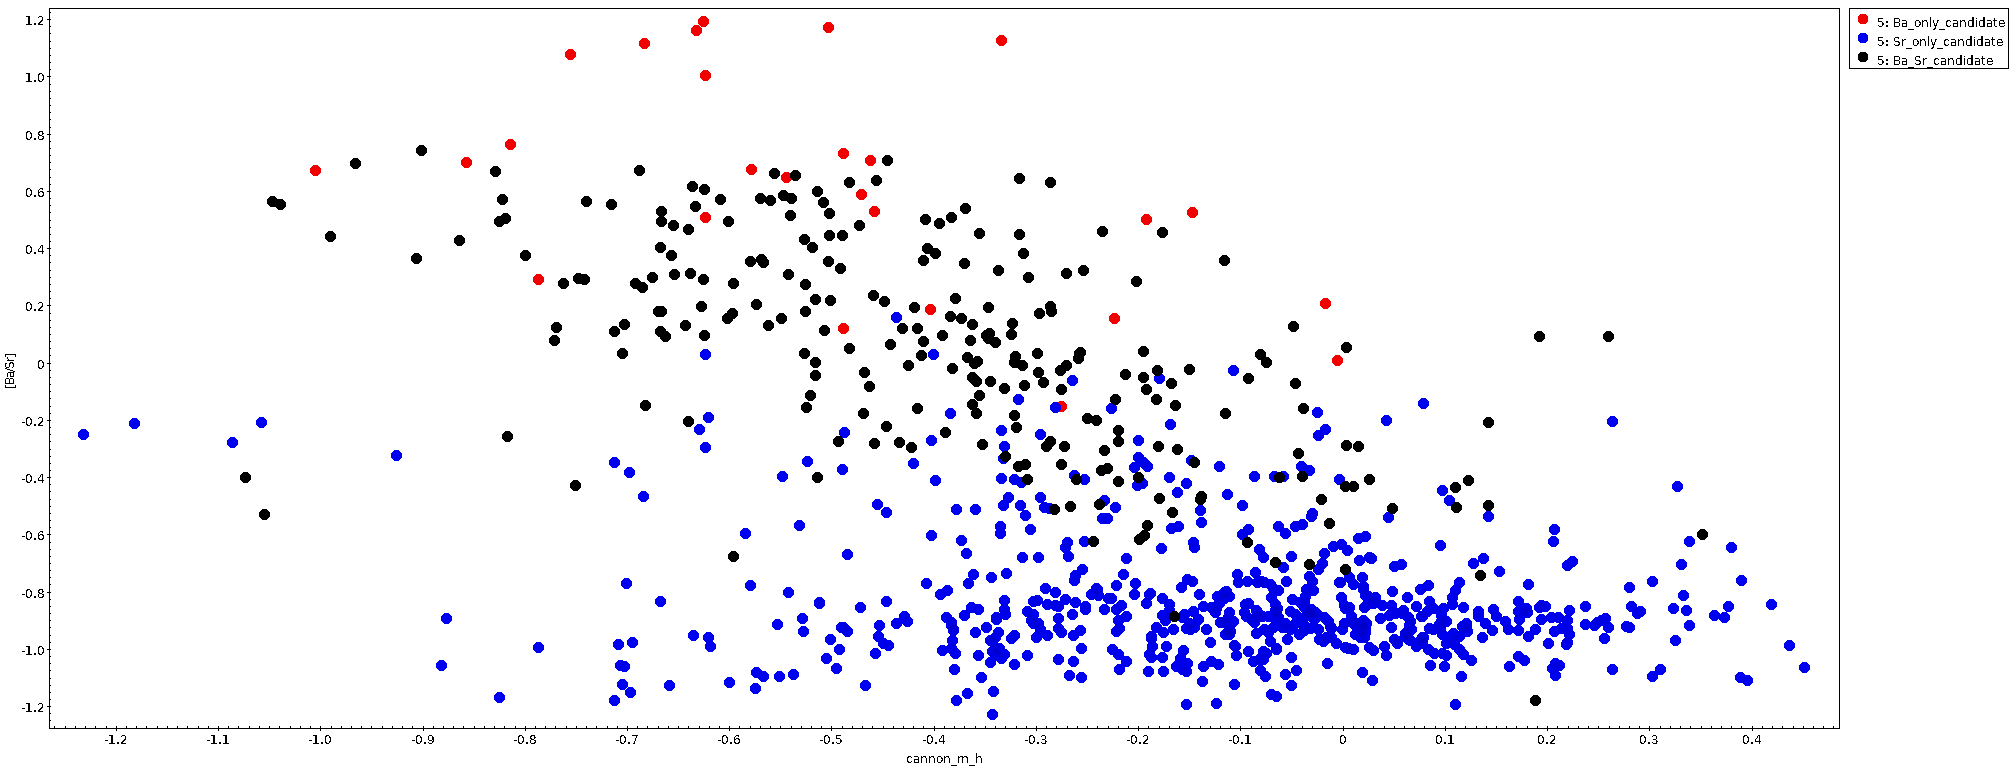
\includegraphics[width=\columnwidth]{basrtest4.png}
    \caption{Metallicities ([Fe/H]; x-axis) and heavy-to-light s-process abundance ratios ([hs/ls], taken as [Ba/Sr]; y-axis) for 257 Barium star candidates. \todo{Add Cristillo yields}}
    \label{fig:figure3}
\end{figure}


\section{Conclusions} \label{sec:con}

We conducted the largest ever search for s-process enhanced stars using the LAMOST second data release. From 454,180 giant stars, we identify 967 s-process candidates including: 257 stars with significant enhancements in barium and strontium (so-called `Barium stars'); 49 stars exhibiting exclusively barium enhancement, and 661 exhibiting exclusively strontium enhancement. This sample size is double the total number of Barium stars known, and represents the largest sample of s-process enhanced stars to date. Nearly all of our Barium candidates are consistent with being disk stars. 

We find 178/257 to show carbon enhancement, consistent with the literature. However, in contrast with previous works, we do not find Barium stars to have significantly higher [Na/Fe] than Milky Way stars. Only 5/257 of our Barium stars show enhancement in Na, and the flux residuals in three of those are likely due to interstellar dust. We suggest that biases between literature sources and systematic effects in measuring [Na/Fe] from stars with low $\log{g}$ contributed to this effect. 

Despite our noisy estimates of [Ba/Fe] and [Sr/Fe] from LAMOST spectra, comparisons with AGB yields indicate that our sample is consistent with a bottom-heavy initial mass function. We encourage follow-up observations with high-resolution spectrographs in order to precisely measure neutron-capture abundances (including [hs/ls] ratios). These data would permit the most detailed comparisons with AGB star yields ever considered.

 

\section*{Acknowledgements}
We thank Alex Ji (Carnegie Observatories) for useful discussions.
A.~R.~C. is supported through an Australian Research Council Discovery Project under grant DP160100637.
A.~Y.~Q.~H. is supported by a Fulbright grant through the German-American Fulbright Commission and a National Science Foundation Graduate Research Fellowship under Grant No. DGE-1144469. 
This research has made use of NASA's Astrophysics Data System.
Guoshoujing Telescope (the Large Sky Area Multi-Object Fiber Spectroscopic Telescope LAMOST) is a National Major Scientific Project built by the Chinese Academy of Sciences. Funding for the project has been provided by the National Development and Reform Commission. LAMOST is operated and managed by the National Astronomical Observatories, Chinese Academy of Sciences.


 
\bibliographystyle{mnras}
%\bibliography{example} % if your bibtex file is called example.bib

\begin{thebibliography}{99}
\bibitem[Alam et al.(2015)]{alam2015} Alam, S., Albareti, F.~D., Allende Prieto, C., et al.\ 2015, \apjs, 219, 12 
\bibitem[\protect\citeauthoryear{Allen \& Barbuy}{2006}]{allen2006}
Allen, D.~M.,\& Barbuy B. 2006, 
A$\&$A, 454, 917
\bibitem[\protect\citeauthoryear{Antipova et al.}{2004}]{antipova2004}
Antipova, L.~I., Boyarchuk, A.~A., Pakhomov, Yu.~V.,\& Panchuk, V.~E. 2004, 
ARep, 48, 597
\bibitem[\protect\citeauthoryear{Bidelman \& Keenan}{1951}]{Bidelman1951}
Bidelman, W.~P. \& Keenan, P.~C. , 1951, ApJ, 114, 473
\bibitem[\protect\citeauthoryear{Bisterzo et al.}{2014}]{bisterzo2014}
Bisterzo, S., et al. 2014, 
ApJ, 787, 10
A$\&$A, 424, 727
\bibitem[Blanco-Cuaresma et al.(2014)]{ispec} Blanco-Cuaresma, S., Soubiran, C., Heiter, U., \& Jofr{\'e}, P.\ 2014, \aap, 569, A111 
\bibitem[\protect\citeauthoryear{Boffin \& Jorissen}{1988}]{boffin1988}
Boffin H, M.~J.,\& Jorissen, A. 1988, 
A$\&$A, 205, 155
\bibitem[\protect\citeauthoryear{B\"ohm-Vitense}{1980}]{bohm1980}
B\"ohm-Vitense, E. 1980, 
ApJ, 239, L79
\bibitem[\protect\citeauthoryear{B\"ohm-Vitense et al.}{1984}]{bohm1984}
B\"ohm-Vitense, E., Nemec, J.,\& Proffitt, C. 1984, 
ApJ, 278, 726
\bibitem[\protect\citeauthoryear{Bovy}{2015}]{bovy2015}
Bovy, J. 2015, 
ApJ, 216, 29
\bibitem[\protect\citeauthoryear{Boyarchuk et al.}{2002}]{boyarchuk2002}
Boyarchuk, A.~A., Pakhomov, Y.~V., Antipova, L.~I.,\& Boyarchuk, M.~E. 2002, 
ARep, 46, 819
\bibitem[\protect\citeauthoryear{Busso et al.}{1999}]{busso1999}
Busso, M., Gallino, R., \& Wasserburg, P.~C. 1999, 
ARA$\&$A, 37, 239
\bibitem[\protect\citeauthoryear{Busso et al.}{2001}]{busso2001}
Busso, M., Gallino, R., Lambert, D.~L., Travaglio, C.\& Smith, V.~V. 2001, 
ApJ, 557, 802
\bibitem[\protect\citeauthoryear{Casey}{2014}]{casey2014}
Casey, A.~R. 2014, 
PhD Thesis, Australian National University
\bibitem[\protect\citeauthoryear{Cristallo et al.}{2015}]{cristallo2015}
Cristallo, S., Straniero, O., Piersanti, L.,\& Gobrecht, D. 2015, 
ApJ, 219, 40
\bibitem[\protect\citeauthoryear{deCastro et al.}{2016}]{decastro2016}
deCastro, D.~B., Pereira, C.~B., Roig, F., Jilinski, E., Drake, N.~A., Chavero, C.,\& Sales Silva, J.~V. 2016, 
MNRAS, 459, 4299
\bibitem[\protect\citeauthoryear{Denissenkov \& Ivanov}{1987}]{denissenkov1987}
Denissenkov P.~A.,\& Ivanov, V.~V. 1987, 
SvAL, 13, 214
\bibitem[\protect\citeauthoryear{Drake \& Pereira}{2008}]{drake2008}
Drake N.,~A.,\& Pereira, C.~B. 2008, 
AJ, 135, 1070
\bibitem[\protect\citeauthoryear{El Eid \& Champagne}{1995}]{el1995}
El Eid, M.~F.,\& Champagne, A.~E. 1995, 
ApJ, 451, 298
\bibitem[\protect\citeauthoryear{Gaia Collaboration et al.}{2016a}]{gaia2016a}
Gaia Collaboration, Brown, A.~G.~A., Vallenari, A., Prusti, T., de Bruijne, J.~H.~J., Mignard, F., Drimmel, R., Babusiaux, C., Bailer-Jones, C.~A.~L.,\& Bastian, U., et al. 2016, 
A$\&$A, 595, A2
\bibitem[\protect\citeauthoryear{Gaia Collaboration et al.}{2016b}]{gaia2016b}
Gaia Collaboration, Prusti, T., de Bruijne, J.~H.~J., Brown, A.~G.~A., Vallenari, A., Babusiaux, C., Bailer-Jones, C.~A.~L., Bastian, U., Biermann, M.,\& Evans, D.~W. et al. 2016, 
A$\&$A, 595, A1
\bibitem[Gustafsson et al.(2008)]{marcs} Gustafsson, B., Edvardsson, B., Eriksson, K., et al.\ 2008, \aap, 486, 951 
\bibitem[\protect\citeauthoryear{Gomez et al.}{1997}]{gomez1997}
Gomez, A.~E., Luri, X., Grenier, S., et al. 1997, 
A$\&$A, 319, 881
\bibitem[\protect\citeauthoryear{Han et al.}{1995}]{han1995}
Han, Z., Eggleton, P.~P., Podsiadlowski, P.,\& Tout, C.~A. 1995, 
MNRAS, 277, 1443
\bibitem[\protect\citeauthoryear{Hernquist}{1990}]{hernquist1990}
Hernquist, L. 1990, 
ApJ, 356, 359
\bibitem[\protect\citeauthoryear{Herwig}{2005}]{herwig2005}
Herwig, F. 2005, 
ARA$\&$A, 43, 435
\bibitem[\protect\citeauthoryear{Ho et al.}{2017}]{ho2017}
Ho, A.~Y.~Q., Ness, M.~K., Hogg, D.~W., Rix, H.-W. Liu, C., Yang, F., Zhang, Y., Hou, Y.,\& Wang, Y. 2017, 
ApJ, 836, 5
\bibitem[\protect\citeauthoryear{Jorissen \& Boffin}{1992}]{jorissen1992}
Jorissen, A.,\& Boffin H, M.~J., 1992, 
Evidences for interaction among wide binary systems: To Ba or not to Ba? In: Duquennoy, A., Mayor, M.,(eds.) Binaries as tracers of stellar formation. Cambridge Univ. Press., p.185
\bibitem[\protect\citeauthoryear{Jorissen et al.}{1993}]{jorissen1993}
Jorissen, A., Frayer, D.~T., Johnson, H.~W., Mayor, M.,\& Smith, V.~V. 1993, 
A$\&$A, 271, 463
\bibitem[\protect\citeauthoryear{Jorissen et al.}{2005}]{jorissen2005}
Jorissen, A., Za$\check{c}$, L., Udry, S., Lindgren, H.,\& Musaev, F.~A. 2005, 
A$\&$A, 441, 1135
\bibitem[\protect\citeauthoryear{Junqueira \& Pereira}{2001}]{junqueira2001}
Junqueira S.,\& Pereira, C.~B. 2001, 
AJ, 122, 360
\bibitem[\protect\citeauthoryear{Karakas}{2016}]{karakas12016}
Karakas, A. 2016, 
SAIt, 87, 229
\bibitem[\protect\citeauthoryear{Karakas \& Lugaro}{2016}]{karakas_lugaro2016}
Karakas, A.~I.,\& Lugaro M. 2016, 
ApJS, 825, 26
\bibitem[\protect\citeauthoryear{Kelson et al.}{2000}]{kelson2000}
Kelson, D.~D., Illingworth, G.~D., van Dokkum, P.~G.,\& Franx, M. 2000, ApJ, 531, 159
\bibitem[\protect\citeauthoryear{Kelson}{2003}]{kelson2003}
Kelson, D.~D. 2003, 
PASP, 115, 688
\bibitem[\protect\citeauthoryear{Kobayashi et al.}{2011}]{kobayashi2011}
Kobayashi, C., Karakas, A., \& Umeda, H. 2011, 
MNRAS, 414, 3231
\bibitem[Kupka et al.(1999)]{vald} Kupka, F., Piskunov, N., Ryabchikova, T.~A., Stempels, H.~C., \& Weiss, W.~W.\ 1999, \aaps, 138, 119 
\bibitem[\protect\citeauthoryear{Little-Marenin \& Little}{1987}]{little1987}
Little-Marenin, I.~R.,\& Little, S.~J. 1987, 
AJ, 93, 1539
\bibitem[\protect\citeauthoryear{Luck \& Heiter}{2007}]{luck2007}
Luck R.~E.,\& Heiter, U. 2007, 
AJ, 133, 2464
\bibitem[\protect\citeauthoryear{Luo et al}{2015}]{luo2015}
Luo, A.~L., Bai, Z.~R., et al. 2015, 
RAA, in press
\bibitem[Maiorca et al.(2011)]{maiorca2011} Maiorca, E., Randich, S., Busso, M., Magrini, L., \& Palmerini, S.\ 2011, \apj, 736, 120 
\bibitem[\protect\citeauthoryear{McClure}{1983}]{mcclure1983}
McClure, R.~D. 1983, 
ApJ, 268, 264
\bibitem[\protect\citeauthoryear{Mennessier et al.}{1997}]{mennessier1997}
Mennessier, M.~O., Luri, X., Figueras, F., et al. 1997, 
A$\&$A, 326, 722
\bibitem[\protect\citeauthoryear{Mishenina et al.}{2006}]{mishenina2006}
Mishenina, T.~V., Bienaym\' e, O., Gorbaneva, T.~I.,\& Charbonnel, C. 2006, 
A$\&$A, 456, 1109
\bibitem[\protect\citeauthoryear{Miyamoto-Nagai}{1975}]{miyamoto1975}
Miyamoto, M,\& Nagai, R. 1975, 
PASJ, 27, 533
\bibitem[\protect\citeauthoryear{NFW}{1997}]{nfw1997}
Navarro, J.~F., Frenk, C.~S.,\& White, S.~D.~M. 1997, 
ApJ, 490, 493
\bibitem[\protect\citeauthoryear{Pereira \& Drake}{2009}]{pereira2009}
Pereira, C.~B.,\& Drake N.,~A. 2009, 
A$\&$A, 496, 791
\bibitem[\protect\citeauthoryear{Pereira et al.}{2011}]{pereira2011}
Pereira, C.~B., Sales Silva, J.,~A., Chavero, C., Roig, F.,\& Jilinski E. 2011, 
A$\&$A, 533, A51
\bibitem[\protect\citeauthoryear{Pourbaix et al.}{2004}]{pourbaix2004}
Pourbaix, D., Tokovinin, A.~A., Batten, A.~H., Fekel, F.~C., Hartkopf, W.~I. et al. 2001, 
\bibitem[\protect\citeauthoryear{Prantzos}{2012}]{prantzos2012}
Prantzos, N. 2012, 
A$\&$A, 542, A67
\bibitem[\protect\citeauthoryear{Price-Whelan}{2017}]{price2017}
Price-Whelan, A.~M. 2017, 
The Journal of Open Source Software, 2, 388
\bibitem[\protect\citeauthoryear{Romano et al.}{2010}]{romano2010}
Romano, D., et al. 2010, 
A$\&$A, 522, A32
\bibitem[\protect\citeauthoryear{Schlafly \& Finkbeiner}{2011}]{schlafly2011}
Schlafly, E.~F.,\& Finkbeiner, D.~P. 2011, 
Apj, 737, 103
\bibitem[\protect\citeauthoryear{Smith \& Wallerstein}{1983}]{smith1983}
Smith, V.~V.,\& Wallerstein, G. 1983, 
ApJ, 273, 742
\bibitem[\protect\citeauthoryear{Smith}{1984}]{smith1984}
Smith, V.~V. 1984, 
A$\&$A, 132, 326
\bibitem[\protect\citeauthoryear{Takeda et al.}{2008}]{takeda2008}
Takeda, Y., Sato, B.~V.,\& Murata, D. 2008, 
AJ, 60, 781
\bibitem[\protect\citeauthoryear{Travaglio et al.}{2001}]{travaglio2001}
Travaglio, C., et al. 2001, 
ApJ, 549, 346
\bibitem[\protect\citeauthoryear{Webbink}{1986}]{webbink1986}
Webbink, R.~F. 1986, 
In: Leung, K.~C., Zhai, D.~S.(eds.) Critical Observations versus Physical Models for Close Binary Systems. Gordon and Breach, New York, p.403
\bibitem[\protect\citeauthoryear{Whitelock et al.}{2013}]{whitelock2013}
Whitelock, P.~A., et al. 2013, 
MNRAS, 428, 2216
\bibitem[Valenti \& Piskunov(1996)]{sme} Valenti, J.~A., \& Piskunov, N.\ 1996, \aaps, 118, 595 
\bibitem[\protect\citeauthoryear{Van der Swaelmen et al.}{2017}]{van2017}
Van der Swaelmen, M., Boffin, H.~M.~J., Jorissen, A.,\& Van Eck, S. 2017, 
A$\&$A, 597, A68






\end{thebibliography}


% Don't change these lines
\bsp	% typesetting comment
\label{lastpage}
\end{document}